\documentclass[12pt,xcolor=dvipsnames%,mathserif%,handout
   ]{beamer}
% \PassOptionsToClass{beamer}{handout}
% \usepackage{pgfpages} 
% \pgfpagesuselayout{4 on 1}[letterpaper,landscape,border shrink=3mm]
\usepackage{amsmath}
\usepackage{helvet}
\usepackage{../inputs/mymacros}
% \usepackage{../inputs/macros}
\usepackage{comment}
\usepackage{xspace}
\usepackage{pifont}
\usepackage[all,cmtip,arrow]{xy}  %for xy-pic fonts
%%macs
%For this presentation, I don't want citations
\renewcommand{\cite}[1]{\relax}
\newcommand{\V}{\ensuremath{\mathcal V}\xspace}
\newcommand{\mbold}[1]{\ensuremath{\mathbf{#1}}\xspace}
\makecs{\mbold}{ABDP}
\newcommand{\exmpl}[1]{{\color{green!50!black} #1}}
\newcommand{\dsize}{\displaystyle}
\DeclareMathOperator{\End}{End}
\DeclareMathOperator{\Var}{Var}
\DeclareMathOperator{\Cg}{Cg}
\DeclareMathOperator{\Sub}{Sub}
\DeclareMathOperator{\Con}{Con}
\DeclareMathOperator{\Rel}{Rel}
\newcommand{\bigpause}{\pause\bigskip}
\DeclareMathOperator{\CSP}{CSP}
\newcommand{\FF}{\mathbb{F}}
\DeclareMathOperator{\Pol}{Pol}
\DeclareMathOperator{\Inv}{Inv}
\renewcommand{\.}{\cdot}
\DeclareMathOperator{\core}{core}
\newcommand{\sA}{\ensuremath{\mathcal{A}}}
\newcommand{\sV}{\ensuremath{\mathcal{V}}}
\newcommand{\sS}{\ensuremath{\mathcal{S}}}
\newcommand{\sR}{\ensuremath{\mathcal{R}}}
\newcommand{\sD}{\ensuremath{\mathcal{D}}}
\newcommand{\bA}{\ensuremath{\mathbf{A}}}
\newcommand{\sF}{\ensuremath{\mathcal{F}}}
\newcommand{\defn}[1]{\textit{#1}}
\renewcommand{\ar}{\ensuremath{\operatorname{ar}}}
 \newcommand{\bR}{\ensuremath{\mathbf{R}}}

\newcommand{\reduc}{\leq_{\text{\textnormal{p}}}}
\newcommand{\equivp}{\equiv_{\text{\textnormal{p}}}}
\newcommand{\NP}{\ensuremath{\mathbb{NP}}\xspace}
\renewcommand{\P}{\ensuremath{\mathbb{P}}\xspace}
\newcommand{\Blue}{\textcolor{blue!50!black}}
\newcommand{\Red}{\textcolor{violet!50!red}}
\newcommand{\Green}{\textcolor{green!55!black}}
\let\origemph=\emph 
\let\origtextbf=\textbf 
%%endmacs
%%
\parskip=10pt
%% Beamer Setup
% \mode<handout>{\beamertemplatesolidbackgroundcolor{black!5}}
\mode<presentation>{
  % \usetheme{Singapore}
   % \usetheme{Frankfurt}
   % \usetheme{Pittsburgh}
   \usetheme{Boadilla}
   % \usetheme{lankton-keynote}
   \usecolortheme{beaver}
  % \useinnertheme[shadow]{rounded}
  \setbeamertemplate{navigation symbols}[only frame symbol]{}
}
% \mode<beamer>
% {%
%   \let\emph=\alert}
%   \renewcommand{\textbf}[1]{{\usebeamercolor[fg]{example text}%
%      \origtextbf{#1}}}
% }
\mode<article>{\usepackage{fullpage}}
%%
%\title{\TeX\ and \LaTeX\ in the Mathematics Department}
%\author{Clifford Bergman}

\renewcommand{\phi}{\ensuremath{\varphi}}
\begin{document}
\title[Algebraic CSP]{Algebraic Approach to Complexity of Constraint Satisfaction Problems}
\author[\url{williamdemeo@gmail.com}]{William DeMeo\\
{\small \url{williamdemeo@gmail.com}}}
%\\[5pt]{\small University of Hawaii}

\date[29 Sep 2016]{Hawaii Logic Seminar\\[10pt]
29 September 2016}

\frame[plain]{\titlepage}

\setbeamercolor{block body example}%
{parent=normal text,use=block title example,bg=block title example.bg!25!bg}

\begin{frame}
\frametitle{What is a CSP?}

  Informally, a \textbf{C}onstraint \textbf Satisfaction \textbf Problem
  consists of
  \begin{itemize}
  \item a list of variables ranging over a finite domain and
  \item a set of constraints on those variables.
  \end{itemize}

  \textbf{Problem:} can we assign values to all the variables so that
  all of the constraints are satisfied?

\end{frame}

\begin{frame}
  \frametitle{Examples}

A system of linear equations is a CSP
\begin{alignat*}4
  a_{11}x_1 &&+ a_{12}x_2 &&+ \cdots &&+ a_{1n}x_n &= b_1 \\
  a_{21}x_1 &&+ a_{22}x_2 &&+ \cdots &&+ a_{2n}x_n &= b_2 \\
  &&\;\vdots \\
  a_{m1}x_1 &&+ a_{m2}x_2 &&+ \cdots &&+ a_{mn}x_n &= b_m \\
\end{alignat*}
\end{frame}

\begin{frame}
  Also, a system of nonlinear equations is a CSP
\begin{alignat*}4
  a_{11}x_1^2x_3 &+ a_{12}x_2x_3x_7 &&+ \cdots &&+ a_{1n}x_4x_n^3 &&= b_1 \\
  a_{21}x_2x_5 &+ a_{22}x_2 &&+ \cdots &&+ a_{2n}x_4^3 &&= b_2 \\
 &&&\vdots \\
  a_{m1}x_3x_5x_8 &+ a_{m2}x_2 &&+ \cdots &&+ a_{mn}x_n &&= b_m \\
\end{alignat*}
\end{frame}

\begin{frame}
  For a fixed $k$, determining whether a graph is $k$-colorable is a CSP
  \begin{center}
    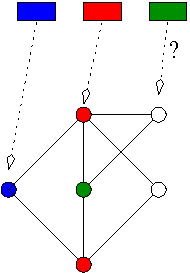
\includegraphics{../inputs/k-col}
%    \fbox{picture suggesting 3-colorability}
  \end{center}
\end{frame}


\begin{frame}
Determining whether a given formula $\phi(x_1,\dots,x_n)$ is satisfiable is a CSP
\bigskip
For example,
\begin{equation*}
\phi(x,y,z) = (x\join y \join \neg z) \meet (\neg x\join y \join \neg z)
\end{equation*}
\pause

is satisfiable. e.g., $(x,y,z) = (0,0,1)$
\end{frame}

\begin{frame}
  \frametitle{Algorithms}
  There is an \emph{efficient} algorithm (Gaussian elimination) for solving any
  linear system.
  That is

% \setbeamercolor{block body example}%
% {parent=normal text,use=block title example,bg=block title example.bg!25!bg}
  \begin{exampleblock}{}
    There is an algorithm that accepts as input a linear system
    and decides whether that system has a solution.

    \smallskip
    The running time of the algorithm is bounded by $f(s)$,
    a \emph{polynomial} in the size $s$ of the system.
  \end{exampleblock}
  \pause

  The \alert{input}, a particular system, is an \alert{instance} of the \alert{problem}
  LINEAR SYSTEM.
  
\end{frame}

\begin{frame}
  Similarly

  % \setbeamercolor{block body example}%
  % {parent=normal text,use=block title example,bg=block title example.bg!25!bg}
  \begin{exampleblock}{}
    There is an algorithm that accepts as input a graph and decides
    whether the graph is 2-colorable.

    \smallskip
    Running time bounded by $f(s)$, a \emph{polynomial} in 
    the size $s$ of the graph.
  \end{exampleblock}

  The \alert{input}, a particular graph, is an \alert{instance} of the \alert{problem} 
  2-COLORABILITY.
\end{frame}


\begin{frame}
  % \setbeamercolor{block body example}%
  % {parent=normal text,use=block title example,bg=block title example.bg!25!bg}
  \begin{exampleblock}{}
  There is an algorithm that accepts as input a formula, $\phi = \phi_1 \meet \phi_2 \meet \cdots \meet \phi_k$ (each $\phi_i$ bijunctive) and decides whether $\phi$ is satisfiable.
  
  \smallskip
  Running time bounded by $f(s)$, a \emph{polynomial} in the length $s$ of a string
  describing $\phi$.
  \end{exampleblock}
  
  The \alert{intput} formula $\phi$ is an \alert{instance} of the \alert{problem} 2-SAT.

  % \bigpause
  We say that all these algorithms run in \alert{polynomial time}.
\end{frame}

\begin{frame}
  No polynomial-time algorithm is known for, NONLINEAR SYSTEM,
  3-COLORABILITY, or 3-SAT.

  \bigpause
  However, any candidate solution to either of these problems can be
  checked in polynomial-time. 

  \bigpause
  Thus these problems are solvable in \alert{nondeterministic polynomial
    time.} 
\end{frame}

\begin{frame}
  Let $X$ and $Y$ be two problems. We write $X \reduc Y$ to indicate that
  $Y$ is at least as hard as $X$.

  \bigpause
  Somewhat more precisely: any algorithm for solving $Y$ can be
  transformed into an algorithm for $X$ without drastically increasing
  its running time.

  \bigpause
  It is possible for $X\reduc Y \reduc X$. In that case, write $X\equivp
  Y$. 

\end{frame}

\begin{frame}
  \P is the class of all problems solvable in polynomial time. Its
  members are called \alert{tractable.}

  \NP is the class of problems solvable in nondeterministic polynomial
  time. 

  \pause
  \begin{itemize}
  \item $\P \sseq \NP$
  \item Both $\P$ and $\NP$ are downsets, i.e., \\
    $Y\in \P \mathrel{\&} X\reduc Y \implies X\in \P$
  \end{itemize}

  \pause
  The maximal members of \NP are called \alert{\NP-complete.} 

  
  3-COLORABILITY, NONLINEAR SYSTEM, and 3-SAT are known to be
  \NP-complete. 
\end{frame}

\begin{frame}
  \frametitle{\$$2^{20}$ question: $\P \overset{?}{=} \NP$.}
  
\includegraphics[scale=.25]{../inputs/cash.png}
  \pause
  \parbox[b][2in][c]{2in}{
      If $\P=\NP$ then all of the above distinctions go away. 
    
     \bigskip

      Most problems we care about can be solved
      efficiently. Just build bigger computers.
    }
      \bigskip
      \pause
      In particular, this talk becomes pointless. So assume $\P\neq \NP$.

  \pause
  \setbeamercolor{block body theorem}%
  {parent=normal text,use=block title theorem,bg=block title theorem.bg!25!bg}
  \begin{exampleblock}{Ladner, 1975 \cite{Ladner1975}} % [Ladner, 1975 \cite{Ladner1975}]
  % \begin{theorem}[Ladner, 1975 \cite{Ladner1975}]
    If $\P \neq \NP$, then there are problems in $\NP\setminus
    \P$ that are not \NP-complete.
  % \end{theorem}
  \end{exampleblock}
\end{frame}

\begin{frame}
  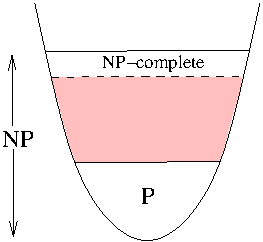
\includegraphics[scale=1.25]{../inputs/complexity}
  \qquad
  \parbox[b][2in][c]{1.5in}{If $\P\neq \NP$ then the pink area is nonempty.}
\end{frame}



%%%%%%%%%%%%%%%%%%%%%%%%%%%%%%%%%%%%%%%%%%%%%%%%%%%%%%%%%%%
%% 1: CSP Intro 1
\begin{frame}
  \frametitle{Oversimplified Definition of CSP}
  
  {\bf Input}
  \begin{itemize}
  \item \emph{variables:} $\sV = \{v_1, v_2, \dots\}$
  \item \emph{domain:}  $\sD$
  \item \emph{constraints:} $C_1, C_2, \dots$
  \end{itemize}
\pause
  \vskip.5cm
  % \underline{Output}
  {\bf Output}
  \begin{itemize}
  \item ``yes'' if there is a \emph{solution}   $f : \sV \rightarrow \sD$ 

    {\small (assigning values to variables and satisfying all $C_i$)}

  \item ``no'' otherwise
  \end{itemize}

\end{frame}





\begin{frame}
  \frametitle{Slightly more formally...}

  Let $D$ be a set, $n$ a positive integer

  An \emph{$n$-ary relation on $D$} is a subset of $D^n$

  \pause
  $\Rel_n(D)$ denotes the set of all $n$-ary relations on $D$

  $\Rel(D) = \bigcup\limits_{n< \omega} \Rel_n(D)$ is the set of all finitary
  relations on $D$
\end{frame}

\begin{frame}  
  \frametitle{Slightly more formal defintion of CSP}

  Let $D$ be a finite set and $\sR \sseq \Rel(D)$

  $\CSP(D,\sR)$ is the following decision problem:

  \textbf{Instance:}
\vskip-3mm
  \begin{itemize}
  \item 
  \alert{variables}: $V=\setof{v_1,\dots,v_n}$ (a finite set) 

\item  \alert{constraints}: $(C_1,\dots,C_m)$ (a finite list) 
  \end{itemize}
  Each $C_i$ is a pair $(\bs_i,\, R_i)$, 
  where \[\bs_i(j) \in V\quad \text{ and } \quad R_i\in \sR\]

  \pause
  \textbf{Question:} Does there exist a \alert{solution}? 

  an assignment $f \colon V\to D$ such that, for all $i\leq m$,
\[(f(\bs_i(1)),\dots,f(\bs_i(p)))\in R_i \]

    % \pause
    % $\CSP(D,\sR)$ always lies in \NP.

%    $\CSP\<D,\sR\>$ is \emph{finitary} if $\sR$ is finite. 
\end{frame}


\begin{frame}
  \frametitle{Example: 3-colorability}

  $D=\{\Red{r},\Green{g},\Blue{b}\}$, \quad $\sR=\{R\}$

  $R =\setof{(x,y)\in D\times D : x\neq y}$

  Then $\CSP(D,\sR)$ is the 3-colorability problem

  \bigskip

    \begin{columns}
      \begin{column}{1.5in}
        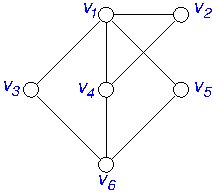
\includegraphics{../inputs/col_csp}
      \end{column}
      \begin{column}{2in}
        $V=\{v_1,\dots,v_6\}$\\
        $\bs_1 = (v_1,v_2)$\\
        $\bs_2 = (v_2,v_4)$\\
        % $\bs_3 = (v_1,v_4)$\\
        % $\bs_4=(v_2,v_4)$\\
        \qquad$\vdots$\\
        $\bs_m = (v_5,v_6)$\\[4pt]
        $R_i = R$ for every $i$.
      \end{column}
    \end{columns}
  \end{frame}

% \begin{comment}
  
\begin{frame}
\frametitle{Example: 2-SAT}
$D=\{0,1\}$\\
For a bijunctive clause $\phi(x,y)$, 
\begin{equation*}
R_\phi= \setof{\<a,b\>\in D^2: \phi(a,b)=1}
\end{equation*}

\pause
\begin{tabular}{cc|c}
 $x$ & $y$ &$x\join y'$  \\
 \hline
0 & 0 & 1\\
\visible<2>{0 & 1 & 0}\\
1 & 0 & 1\\
1 & 1 & 1
\end{tabular}
\uncover<3->{\qquad \parbox{2.5in}{So $R_{x\join y'} = \{\<00\>,\,\<10\>,\,\<11\>\}%=\\ \{0,1\}^2-\{\<01\>\}
$}}


\uncover<4->{$\displaystyle\sR=\{R_{x\join y},\, R_{x\join y'},\,R_{x'\join y},\, R_{x'\join y'}\}$}

\uncover<5->{
2-SAT is $\CSP(D,\sR)$}
\end{frame}

\begin{comment}
  
\begin{frame}
\frametitle{Example: Horn-SAT}
\alert{Horn formula:}\\
 $(x_0 \meet x_1 \meet \cdots \meet x_{i-1} \meet x_{i+1} \meet \cdots \meet x_{n-1}) \rightarrow x_i$\\[6pt]
\alert{Equivalently:}\\
 $x_0' \join x_1' \join \dots x_{i-1}' \join x_i \join \cdots \join x_{n-1}'$

\bigpause
Corresponding relation $\gamma^n_i = \{0,1\}^n-\{\<111\dots0\dots111\>\}$

\bigpause
Horn-SAT is $\CSP(D,\Gamma)$\\
$D=\{0,1\}$,\quad $\Gamma=\setof{\gamma^n_i : 0\leq i <n}$
\end{frame}

\end{comment}

\begin{frame}
  \frametitle{Schaefer's Dichotomy}

  \begin{exampleblock}{Schaefer, 1978 \cite{Schaefer1978}}
    Let $D=\{0,1\}$. There are six families $\sR_0,
  \dots, \sR_5$ such that
  \begin{equation*}
    \CSP(D,\sR) \in \P \iff \sR \sseq \sR_i, \text{some $i< 6$}
  \end{equation*}
  Otherwise $\CSP(D,\sR)$ is $\NP$-complete.
\end{exampleblock}
% \end{theorem}
\end{frame}

\begin{frame}
{\large The six families}
$\sR_0 = \setof{R : \<0,0,\dots,0\>\in R}$ (``All False'')\\[2pt]
$\sR_1 = \setof{R : \<1,1,\dots,1\>\in R}$ (``All True'')\\[2pt]
$\sR_2 = \{R_{x\join y},\, R_{x\join y'},\,R_{x'\join y},\, R_{x'\join y'}\}$ (bijunctive)\\[2pt]
$\sR_3 = \Gamma$ (Horn)\\[2pt]
$\sR_4 = \Gamma^\partial$ (dual-Horn)\\[2pt]
$\sR_5$ (affine, i.e., linear system over $\FF_2$)
\end{frame}


\begin{frame}
  \frametitle{Two Motivating Questions}

  \begin{enumerate}
  \item \alert{Dichotomy Conjecture}\\ Every $\CSP(D,\sR)$ either
    lies in \P\ or is $\NP$-complete.

    \pause

  \item \alert{Tractability Problem}\\ Characterize those CSPs that lie in \P.
  \end{enumerate}
  
  \pause
  What would a characterization look like? What language could we use?
\end{frame}
% \begin{comment}
  
\begin{frame}
\frametitle{Why is 2-SAT tractable, but 3-SAT is not?}

2-SAT: $\sR_2=\{R_{x\join y},\,R_{x\join y'},\, R_{x'\join y},\, R_{x'\join y'}\} $

\smallskip
3-SAT: $\Lambda=\{\lambda_0,\lambda_1,\dots, \lambda_7\}$

\pause
\begin{equation*}
M(x,y,z) = \begin{cases}
	0 \quad&\text{if at least 2 of $x,y,z$ equal 0}\\
	1 &\text{otherwise}
	\end{cases}
\end{equation*}
``Majority Operation''

\pause
$M$ preserves each $R\in \sR_2$:
\begin{equation*}
\begin{matrix}
\<a_1, &b_1\> &\in R\\
\<a_2, &b_2\> &\in R\\
\<a_3, &b_3\> &\in R \text{ implies}\\
\<M(a_1,a_2,a_3), &M(b_1,b_2,b_3)\> &\in R
\end{matrix}
\end{equation*}

\end{frame}

\begin{frame}
But $M$ fails to preserve each $\lambda\in \Lambda$

\medskip
For example, with $\lambda=\lambda_{x\join y\join z'}=\{0,1\}^3-\{\<001\>\}$ 

\begin{align*}
\<1,0,0\> &\in \lambda\\
\<0,0,1\> &\in \lambda\\
\<0,1,1\> &\in \lambda \text{ but}\\
\<0,0,1\> &\notin \lambda
\end{align*}

\end{frame}
% \end{comment}

\begin{frame}
  \frametitle{Polymorphisms}

  \begin{exampleblock}{Definition}
    Let $R \in \Rel_k(D)$ and $f\: D^n \to D$. We say 
    \emph{$f$ preserves $R$} if
    \begin{equation*}
      \begin{split}
        (a_{11}, \dots, a_{1k}),&\dots, (a_{n1},\dots, a_{nk}) \in
        R \implies\\ 
        &\bigl( f(a_{11},\dots, a_{n1}), \dots, f(a_{1k},\dots,a_{nk})
        \bigr) \in R
    \end{split}
    \end{equation*}
  \end{exampleblock}
% \end{definition}

  \begin{overprint}
  \onslide<2|handout:0>
  $f$ is an \emph{$n$-ary operation} on $D$.
  % 
  \onslide<3|handout:1>
    \begin{equation*}
      \newcommand\flab{\scriptstyle{f}}
      \begin{matrix} a_{11} & a_{12} & \dots & a_{1k} & \in & R \\
        a_{21} & a_{22} & \dots & a_{2k} & \in & R \\
        \vdots  & \vdots &       &\vdots  &     & \vdots \\
        a_{n1} & a_{n2} & \dots & a_{nk} & \in & R \\
        \downarrow\flab &\downarrow\flab &  & \downarrow\flab \\
        \star  & \star  & \dots & \star  & \in & R
      \end{matrix}
    \end{equation*}
  \end{overprint}
\end{frame}

\begin{frame}
  % \begin{definition}
  \begin{exampleblock}{Definition}
    Let $\sR$ be a set of relations on $D$.

    \bigskip
    \emph{$\Pol(\sR)$} is the set of operations preserving
    all members of $\sR$. 

    \bigskip
    These are the \alert{polymorphisms} of  $\sR$. 

    \bigpause

    Let $F$ be a set of operations on $D$. 

    \bigskip
    \emph{$\Inv(F)$} is the set of relations preserved by all operations in $F$.
  \end{exampleblock}
% \end{definition}
  
  \bigpause
Important point: \emph{$(D,\Pol(\sR))$ is an algebraic structure}

\end{frame}

\begin{frame}
  \begin{exampleblock}{Theorem}
  % \begin{theorem}
    Let $\sS, \sR \sseq \Rel(D)$. Then
    \begin{equation*}
      \Pol(\sS) \sseq \Pol(\sR) \implies \CSP(\sR) \reduc
      \CSP(\sS). 
    \end{equation*}
  \end{exampleblock}

\pause
Thus, the richer the algebraic structure, the easier the corresponding CSP
\end{frame}
% \begin{comment}
  
\begin{frame}
Schaefer proved that on $D=\{0,1\}$, there are 4 key polymorphisms:

\begin{center}
$M(x,y,z)$ (majority)\\
$x\meet y$\\
$x\join y$\\
$P(x,y,z) =x\oplus y \oplus z = x-y+z$
\end{center}

\bigskip
$(\{0,1\},\sR)$ is tractable iff one of these is a polymorphism of $\sR$

\bigpause
(Un)fortunately, things are more complicated when $\card{D}>2$.
\end{frame}

% \end{comment}

\begin{frame}
\frametitle{Galois Connection}
  One can go back and forth between relational and algebraic structures

  \begin{center}
    \begin{tabular}{ccc}
      \origtextbf{Relational} & &\origtextbf{Algebraic}  \\
      % \origtextbf{Structures} & &\origtextbf{Structures}  \\
      $(D,\sR)$ & $\longrightarrow$ & $(D,\Pol(\sR))$ \\[2pt]
      $(D, \Inv(F))$ & $\longleftarrow$ &$(D,F)$
    \end{tabular}
  \end{center}

  $\CSP(D,\sR) \equivp \CSP(D,\Inv(\Pol(\sR)))$

  \bigpause
  Perhaps expressive power of algebra can help classify CSPs.

  \end{frame}

% \begin{comment}
  
\begin{frame}
\frametitle{The Relational Clone}
For a set $\sR$ of relations on $D$, let $\<\sR\> =
\Inv\bigl(\Pol(\sR)\bigr)$.

$\<\sR\>$ is called the \alert{relational clone} generated by $\sR$.

It coincides with the set of relations definable from $\sR$ by\\
 \emph{primitive positive formulas}.

\pause
$\phi(x_1,\dots,x_n)=(\exists y_1)(\exists y_2)\cdots(\exists y_m)\bigl(R_1(z_{1_1},\dots,z_{1_k}) \meet \dots \meet R_t(z_{t_1},\dots,z_{t_j})\bigr)$

Here $R_1\dots,R_t \in \sR$ and every $z_{i_j} \in \{x_1,\dots,x_n,y_1,\dots,y_m\}$
\end{frame}
% \end{comment}



\begin{frame}
  \frametitle{Algebraic Facts}

  For an algebra $\bA = \<A, F\>$ define 

  \[\CSP(\A) = \CSP(A, \Inv(F))\]

  \pause

  Let \A\ and \B\ be algebras

  $\B \text{ a subalgebra of \A} \implies \CSP(\B) \reduc \CSP(\A)$.

  $\B \text{ a homomorphic image of \A}\implies \CSP(\B) \reduc
  \CSP(\A)$. 
  
  $\CSP(\A^n) \equivp \CSP(\A)$

\end{frame}


\begin{frame}
  \begin{exampleblock}{Bulatov, Jeavons, Krokhin, 2000
    \cite{BulatovKrokhinJeavons2000}}
  % \begin{theorem}[Bulatov, Jeavons, Krokhin, 2000
    % \cite{BulatovKrokhinJeavons2000}]
    If $(D,\sR)$ is a ``core'' and every polymorphism is essentially unary,
    then $\CSP(\sR)$ is \NP-complete.
  % \end{theorem}
  \end{exampleblock}

  $f$ is \emph{essentially unary} if $f(x_1,\dots,x_n) = g(x_j)$ for
  some unary $g$ and some $j\leq n$.

 \pause
  \begin{exampleblock}{Corollary}
 % \begin{corollary}
    3-COLORABILITY, NONLINEAR SYSTEM, and 3-SAT are \NP-complete.
  % \end{corollary}
  \end{exampleblock}

\end{frame}


\begin{frame}
 
  \textbf{Informal reformulation of the dichotomy conjecture}\\
  If \A\ has some
  kind of decent algebraic structure then $\CSP(\A) \in \P$ otherwise
  $\CSP(\A)$ is \NP-complete.
\end{frame}

\begin{frame}
  % \begin{definition}
  \begin{exampleblock}{Definition}
    Let $n>1$. An $n$-ary operation $f$ is called a \emph{weak
      near-unanimity operation} if 
       \begin{equation*}
       \begin{gathered}
       f(x,x,\dots,x) = x \text{ and}\\
    f(y,x,x,x,\dots,x) = f(x,y,x,x,\dots,x) = \cdots\\
    = f(x,x,\dots,x,y)
  \end{gathered}
  \end{equation*}
  % \end{definition}
\end{exampleblock}  
Note: no essentially unary operation is WNU
\end{frame}

\begin{frame}
  \begin{exampleblock}{Bulatov, Larose, Z\'adori, McKenzie, Mar\'oti}
  % \begin{theorem}[Bulatov, Larose, Z\'adori, McKenzie, Mar\'oti
  %   \cite{BulatovJeavonsKrokhin2005,LaroseZadori2003,%
  %   MarotiMcKenzie2008}]
    If $\sR$ is a core and $\Pol(\sR)$ has no WNU operation
    then $\CSP(\sR)$ is \NP-complete.    
  % \end{theorem}
  \end{exampleblock}
\end{frame}


\begin{frame}
  \frametitle{Reformuated Dichotomy Conjecture}

  Let $\sR$ be a core. Then $\CSP(\sR)$ is tractable if and only
  if it has a WNU polymorphism. Otherwise, it is \NP-complete. 

  \bigskip
  \begin{overprint}
    \onslide<2|handout:0> \centering{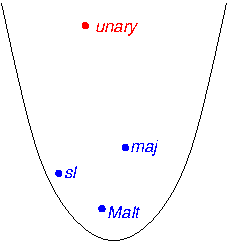
\includegraphics{../inputs/dichotomy1}}
    \onslide<3|handout:0> \centering{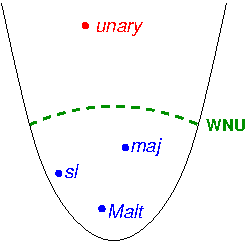
\includegraphics{../inputs/dichotomy2}}
    \onslide<4|handout:0> \centering{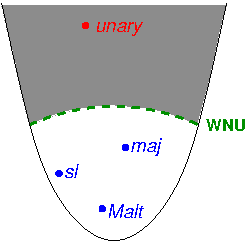
\includegraphics{../inputs/dichotomy3}}
    \onslide<5-|handout:1>
    \begin{exampleblock}{Supporting Examples}
      \begin{itemize}
      \item 2-SAT, 2-COLARABILITY, LINEAR SYSTEM have a WNU.
      
             \item<6-> Let \A\ be an abelian group, $n=|A|$. Choose
        integers $k, l$ with $kl \equiv 1 \pmod n$. Then
        \begin{equation*}
          f(x_1,\dots,x_k) = l(x_1+\cdots + x_k)
        \end{equation*}
        is a WNU operation.
      \end{itemize}
    \end{exampleblock}
  \end{overprint}
\end{frame}

\begin{frame}
\frametitle{Two General Techniques for Tractable Algorithms}
%\begin{enumerate}
\begin{exampleblock}{Method 1}
If $\Pol(\sR)$ contains a ``cube operation'' then $\CSP(\sR)\in \P$
%\end{enumerate}
\end{exampleblock}

\pause
Examples of cube operations: 

$P(x,y,z) = x-y+z$\\
$M(x,y,z) = \text{majority}$

Essentially a generalization of Gaussian elimination. 

Algebras with a cube operation possess ``few subpowers''. This algebraic property is used to prove that the algorithm terminates in polynomial time.

\end{frame}

\begin{frame}
\begin{exampleblock}{Method 2}
If $\Pol(\sR)$ contains WNU operations $v(x,y,z)$ and $w(x,y,z,u)$ satisfying $v(y,x,x)= w(y,x,x,x)$, then $\CSP(\sR)\in \P$.
\end{exampleblock}

\pause
Examples: majority, semilattice 

Algebras with these operations have a property called ``congruence meet-semidistributivity.'' 

\end{frame}

\begin{frame}
\frametitle{Current State of Affairs}
The two general techniques do not cover all cases of a WNU. What to do next? 

\medskip
Two possible directions:
\begin{enumerate}
\item Find a completely new algorithm.
\item Combine the two existing algorithms.
\end{enumerate}

I am exploring both  approaches.
\end{frame}


\end{document}



\begin{frame}
  \frametitle{Overcomplicated Definition of CSP}

  $\bA = (A, \sF)$ is a finite idempotent algebra,
  $\Sub(\bA)$ is all subuniverses of $\bA$.

  {\it In this talk} $\CSP(\bA)$ denotes the following decision problem:

   An \alert{instance of degree} $n$ of $\CSP(\bA)$ is the tuple $\<\sV, \sA, \sS, \sR\>$ 
   \begin{itemize}
   \item \emph{variables} $\sV = \{0, 1, \dots, n-1\}$;
   \item \emph{domains} $\sA = \{\bA_0, \bA_1, \dots, \bA_{n-1}\} \subset \Sub(\bA)$  (one for each variable)
   \item \emph{scope functions} $\sS = (\bs_0, \bs_1, \dots, \bs_{p-1})$ 
     with \emph{constraint arities} $\ar(\sS) = (m_0, m_1, \dots, m_{p-1})$
   \item \emph{constraint relations} $\sR = (\bR_0, \bR_1, \dots, \bR_{p-1})$, where
     \[\bR_i \leq \bA_{\bs_i(0)} \times \bA_{\bs_i(1)}\times \cdots \times \bA_{\bs_i(m_i-1)}.\]
   \end{itemize}
 \end{frame}  
 % \bigskip
  
%   A \alert{solution} to $\<\sV, \sA, \sS, \sR\>$ is an assignment
%   $f: \sV \to A$ of values to variables that satisfies all constraints. That is,
%   \[f\in \myprod_{\sV}A_j
%     \quad  \text{and} \quad 
%     \Proj_{\bs_i} f \in \bR_i, \;\text{ for each $0\leq i < p$.}
%   \]

%   \pause
%   {\bf Notation:} $\nn = \{0,1,\dots, n-1\}$, so the $i$-th scope
%   has type $\bs_i : \mm_i \to \nn$ and
%   \[ \Proj_{\bs_i} f  = f \circ \bs_i \]
% \end{frame}





%%% Local Variables: 
%%% mode: latex
%%% TeX-master: t
%%% End: 
